%!TEX root = ../icip_jseo.tex
% -*- root: ../icip_jseo.tex -*-

\section{Introduction}
\label{sec:intro}

Image matching is a fundamental problem in a variety of computer vision applications, including simultaneous localization and mapping\cite{chang_p-slam:_2007,davison_monoslam:_2007}, object recognition\cite{nister_scalable_2006}, panorama stitching\cite{brown_recognising_2003,wagner_real-time_2010}, augmented reality\cite{klein_parallel_2007,wagner_multiple_2009}, and visual odometry\cite{cheng_visual_2006,nister_visual_2004}. To enhance the image matching quality in various environments, many related techniques have been proposed, such as keypoint-based local matching, histogram-based global matching\cite{le_improving_2013,goncalves_hairis:_2011}, color-based matching\cite{mehtre_color_1995,kankanhalli_cluster-based_1996}, and template-based matching\cite{korman_fast-match:_2013}, etc. Among them, keypoint detection and matching has created great interest since it can provide relatively high matching quality against severe occlusion and do not require segmentation for regions of interest. Also, recent work has concentrated on making invariant to image transformation with low computing power\cite{carrera_robust_2007,mikolajczyk_performance_2005}.

The overall flowchart of keypoint matching and recognition is shown in Fig. \ref{fig:on_offline_process}. These procedure can be divided into two main phases: offline (training) and online (testing) procedure. Offline learning is prerequisite to online matching process. In offline learning phase, a set of reference images to be recognized is analyzed and stored as as types of descriptors in a database. In online learning phase, a newly captured image is analyzed and compared with the reference images in the database to find a nearest reference image. In each phase, common procedures for matching are keypoint detection, description, and matching. To analyze training images, at first, keypoints are detected from the images. Then, from those keypoints, local textures are analyzed and described. In this procedure, to provide robustness against rotation, scale, perspective transform, descriptors are constructed. Then, to be used in online phase, efficient matching structures, as databases, are constructed, such as partitioning trees\cite{arya_optimal_1998,beis_shape_1997,muja_fast_2012}, hashing\cite{salakhutdinov_semantic_2009,gionis_similarity_1999,lv_multi-probe_2007}. In the online matching phase, the database is used to find the most similar corresponding keypoints pair with a given query image. To find the most similar keypoint pairs, with given a query image, keypoints are detected, detected keypoints are described about local texture, and compared with the preconstructed database.

\begin{figure}[hb!]
\centering
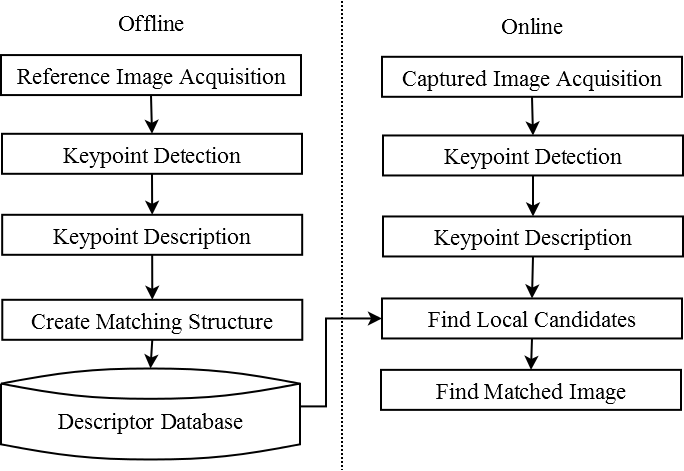
\includegraphics[width=1.0\columnwidth]{introduction/process}
\caption{Overall process of conventional keypoint-based matching}
\label{fig:on_offline_process}
\end{figure}

Conventional keypoint matching methods stores almost every keypoints which are detected by keypoint detection process. Keypoint detection processes are designed to extract repeatable keypoints and robust against arbitrary image transformation. Then, detected keypoints are independent to the follow matching procedures, and do not reflect quality of descriptors. Therefore, as seen Fig.  some keypoints are not distinguishable, and they tend to cause inter-keypoint confusion and miss matching. \texttt{bad keypoint 이미지 추가} Also, those detected keypoints are stored in database and are compared with keypoints in query images in every frame while matching. Then, it decreases the speed of matching. To overcome these problem, in offline learning procedure, detected keypoints are evaluated with respect to proposed matching quality criteria and filtered by the goodness score. With this filtering method, only a small subset of keypoints is stored in the database. Accordingly, it provides more improved matching performance with faster matching speed.

\begin{figure}[ht!]
\centering
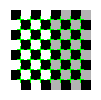
\includegraphics[width=0.5\columnwidth]{introduction/checkerboard}
\caption{Example of high repeatable but poor distinguishable keypoints. Conventional keypoint matching systems do not consider the discriminability of keypoints, so these keypoints usually stored and negatively affected matching.}
\label{fig:example_of_bad_features}
\end{figure}